% Generated by Sphinx.
\def\sphinxdocclass{report}
\documentclass[letterpaper,10pt,english]{sphinxmanual}
\usepackage[utf8]{inputenc}
\DeclareUnicodeCharacter{00A0}{\nobreakspace}
\usepackage{cmap}
\usepackage[T1]{fontenc}
\usepackage{babel}
\usepackage{times}
\usepackage[Bjarne]{fncychap}
\usepackage{longtable}
\usepackage{sphinx}
\usepackage{multirow}

\addto\captionsenglish{\renewcommand{\figurename}{Fig. }}
\addto\captionsenglish{\renewcommand{\tablename}{Table }}
\floatname{literal-block}{Listing }



\title{Delta Stepping Algorithm in Parallel : A beginner approach. Documentation}
\date{May 17, 2016}
\release{0.0.1}
\author{Ivan Felipe Rodriguez Rodriguez}
\newcommand{\sphinxlogo}{}
\renewcommand{\releasename}{Release}
\makeindex

\makeatletter
\def\PYG@reset{\let\PYG@it=\relax \let\PYG@bf=\relax%
    \let\PYG@ul=\relax \let\PYG@tc=\relax%
    \let\PYG@bc=\relax \let\PYG@ff=\relax}
\def\PYG@tok#1{\csname PYG@tok@#1\endcsname}
\def\PYG@toks#1+{\ifx\relax#1\empty\else%
    \PYG@tok{#1}\expandafter\PYG@toks\fi}
\def\PYG@do#1{\PYG@bc{\PYG@tc{\PYG@ul{%
    \PYG@it{\PYG@bf{\PYG@ff{#1}}}}}}}
\def\PYG#1#2{\PYG@reset\PYG@toks#1+\relax+\PYG@do{#2}}

\expandafter\def\csname PYG@tok@gd\endcsname{\def\PYG@tc##1{\textcolor[rgb]{0.63,0.00,0.00}{##1}}}
\expandafter\def\csname PYG@tok@gu\endcsname{\let\PYG@bf=\textbf\def\PYG@tc##1{\textcolor[rgb]{0.50,0.00,0.50}{##1}}}
\expandafter\def\csname PYG@tok@gt\endcsname{\def\PYG@tc##1{\textcolor[rgb]{0.00,0.27,0.87}{##1}}}
\expandafter\def\csname PYG@tok@gs\endcsname{\let\PYG@bf=\textbf}
\expandafter\def\csname PYG@tok@gr\endcsname{\def\PYG@tc##1{\textcolor[rgb]{1.00,0.00,0.00}{##1}}}
\expandafter\def\csname PYG@tok@cm\endcsname{\let\PYG@it=\textit\def\PYG@tc##1{\textcolor[rgb]{0.25,0.50,0.56}{##1}}}
\expandafter\def\csname PYG@tok@vg\endcsname{\def\PYG@tc##1{\textcolor[rgb]{0.73,0.38,0.84}{##1}}}
\expandafter\def\csname PYG@tok@m\endcsname{\def\PYG@tc##1{\textcolor[rgb]{0.13,0.50,0.31}{##1}}}
\expandafter\def\csname PYG@tok@mh\endcsname{\def\PYG@tc##1{\textcolor[rgb]{0.13,0.50,0.31}{##1}}}
\expandafter\def\csname PYG@tok@cs\endcsname{\def\PYG@tc##1{\textcolor[rgb]{0.25,0.50,0.56}{##1}}\def\PYG@bc##1{\setlength{\fboxsep}{0pt}\colorbox[rgb]{1.00,0.94,0.94}{\strut ##1}}}
\expandafter\def\csname PYG@tok@ge\endcsname{\let\PYG@it=\textit}
\expandafter\def\csname PYG@tok@vc\endcsname{\def\PYG@tc##1{\textcolor[rgb]{0.73,0.38,0.84}{##1}}}
\expandafter\def\csname PYG@tok@il\endcsname{\def\PYG@tc##1{\textcolor[rgb]{0.13,0.50,0.31}{##1}}}
\expandafter\def\csname PYG@tok@go\endcsname{\def\PYG@tc##1{\textcolor[rgb]{0.20,0.20,0.20}{##1}}}
\expandafter\def\csname PYG@tok@cp\endcsname{\def\PYG@tc##1{\textcolor[rgb]{0.00,0.44,0.13}{##1}}}
\expandafter\def\csname PYG@tok@gi\endcsname{\def\PYG@tc##1{\textcolor[rgb]{0.00,0.63,0.00}{##1}}}
\expandafter\def\csname PYG@tok@gh\endcsname{\let\PYG@bf=\textbf\def\PYG@tc##1{\textcolor[rgb]{0.00,0.00,0.50}{##1}}}
\expandafter\def\csname PYG@tok@ni\endcsname{\let\PYG@bf=\textbf\def\PYG@tc##1{\textcolor[rgb]{0.84,0.33,0.22}{##1}}}
\expandafter\def\csname PYG@tok@nl\endcsname{\let\PYG@bf=\textbf\def\PYG@tc##1{\textcolor[rgb]{0.00,0.13,0.44}{##1}}}
\expandafter\def\csname PYG@tok@nn\endcsname{\let\PYG@bf=\textbf\def\PYG@tc##1{\textcolor[rgb]{0.05,0.52,0.71}{##1}}}
\expandafter\def\csname PYG@tok@no\endcsname{\def\PYG@tc##1{\textcolor[rgb]{0.38,0.68,0.84}{##1}}}
\expandafter\def\csname PYG@tok@na\endcsname{\def\PYG@tc##1{\textcolor[rgb]{0.25,0.44,0.63}{##1}}}
\expandafter\def\csname PYG@tok@nb\endcsname{\def\PYG@tc##1{\textcolor[rgb]{0.00,0.44,0.13}{##1}}}
\expandafter\def\csname PYG@tok@nc\endcsname{\let\PYG@bf=\textbf\def\PYG@tc##1{\textcolor[rgb]{0.05,0.52,0.71}{##1}}}
\expandafter\def\csname PYG@tok@nd\endcsname{\let\PYG@bf=\textbf\def\PYG@tc##1{\textcolor[rgb]{0.33,0.33,0.33}{##1}}}
\expandafter\def\csname PYG@tok@ne\endcsname{\def\PYG@tc##1{\textcolor[rgb]{0.00,0.44,0.13}{##1}}}
\expandafter\def\csname PYG@tok@nf\endcsname{\def\PYG@tc##1{\textcolor[rgb]{0.02,0.16,0.49}{##1}}}
\expandafter\def\csname PYG@tok@si\endcsname{\let\PYG@it=\textit\def\PYG@tc##1{\textcolor[rgb]{0.44,0.63,0.82}{##1}}}
\expandafter\def\csname PYG@tok@s2\endcsname{\def\PYG@tc##1{\textcolor[rgb]{0.25,0.44,0.63}{##1}}}
\expandafter\def\csname PYG@tok@vi\endcsname{\def\PYG@tc##1{\textcolor[rgb]{0.73,0.38,0.84}{##1}}}
\expandafter\def\csname PYG@tok@nt\endcsname{\let\PYG@bf=\textbf\def\PYG@tc##1{\textcolor[rgb]{0.02,0.16,0.45}{##1}}}
\expandafter\def\csname PYG@tok@nv\endcsname{\def\PYG@tc##1{\textcolor[rgb]{0.73,0.38,0.84}{##1}}}
\expandafter\def\csname PYG@tok@s1\endcsname{\def\PYG@tc##1{\textcolor[rgb]{0.25,0.44,0.63}{##1}}}
\expandafter\def\csname PYG@tok@gp\endcsname{\let\PYG@bf=\textbf\def\PYG@tc##1{\textcolor[rgb]{0.78,0.36,0.04}{##1}}}
\expandafter\def\csname PYG@tok@sh\endcsname{\def\PYG@tc##1{\textcolor[rgb]{0.25,0.44,0.63}{##1}}}
\expandafter\def\csname PYG@tok@ow\endcsname{\let\PYG@bf=\textbf\def\PYG@tc##1{\textcolor[rgb]{0.00,0.44,0.13}{##1}}}
\expandafter\def\csname PYG@tok@sx\endcsname{\def\PYG@tc##1{\textcolor[rgb]{0.78,0.36,0.04}{##1}}}
\expandafter\def\csname PYG@tok@bp\endcsname{\def\PYG@tc##1{\textcolor[rgb]{0.00,0.44,0.13}{##1}}}
\expandafter\def\csname PYG@tok@c1\endcsname{\let\PYG@it=\textit\def\PYG@tc##1{\textcolor[rgb]{0.25,0.50,0.56}{##1}}}
\expandafter\def\csname PYG@tok@kc\endcsname{\let\PYG@bf=\textbf\def\PYG@tc##1{\textcolor[rgb]{0.00,0.44,0.13}{##1}}}
\expandafter\def\csname PYG@tok@c\endcsname{\let\PYG@it=\textit\def\PYG@tc##1{\textcolor[rgb]{0.25,0.50,0.56}{##1}}}
\expandafter\def\csname PYG@tok@mf\endcsname{\def\PYG@tc##1{\textcolor[rgb]{0.13,0.50,0.31}{##1}}}
\expandafter\def\csname PYG@tok@err\endcsname{\def\PYG@bc##1{\setlength{\fboxsep}{0pt}\fcolorbox[rgb]{1.00,0.00,0.00}{1,1,1}{\strut ##1}}}
\expandafter\def\csname PYG@tok@mb\endcsname{\def\PYG@tc##1{\textcolor[rgb]{0.13,0.50,0.31}{##1}}}
\expandafter\def\csname PYG@tok@ss\endcsname{\def\PYG@tc##1{\textcolor[rgb]{0.32,0.47,0.09}{##1}}}
\expandafter\def\csname PYG@tok@sr\endcsname{\def\PYG@tc##1{\textcolor[rgb]{0.14,0.33,0.53}{##1}}}
\expandafter\def\csname PYG@tok@mo\endcsname{\def\PYG@tc##1{\textcolor[rgb]{0.13,0.50,0.31}{##1}}}
\expandafter\def\csname PYG@tok@kd\endcsname{\let\PYG@bf=\textbf\def\PYG@tc##1{\textcolor[rgb]{0.00,0.44,0.13}{##1}}}
\expandafter\def\csname PYG@tok@mi\endcsname{\def\PYG@tc##1{\textcolor[rgb]{0.13,0.50,0.31}{##1}}}
\expandafter\def\csname PYG@tok@kn\endcsname{\let\PYG@bf=\textbf\def\PYG@tc##1{\textcolor[rgb]{0.00,0.44,0.13}{##1}}}
\expandafter\def\csname PYG@tok@o\endcsname{\def\PYG@tc##1{\textcolor[rgb]{0.40,0.40,0.40}{##1}}}
\expandafter\def\csname PYG@tok@kr\endcsname{\let\PYG@bf=\textbf\def\PYG@tc##1{\textcolor[rgb]{0.00,0.44,0.13}{##1}}}
\expandafter\def\csname PYG@tok@s\endcsname{\def\PYG@tc##1{\textcolor[rgb]{0.25,0.44,0.63}{##1}}}
\expandafter\def\csname PYG@tok@kp\endcsname{\def\PYG@tc##1{\textcolor[rgb]{0.00,0.44,0.13}{##1}}}
\expandafter\def\csname PYG@tok@w\endcsname{\def\PYG@tc##1{\textcolor[rgb]{0.73,0.73,0.73}{##1}}}
\expandafter\def\csname PYG@tok@kt\endcsname{\def\PYG@tc##1{\textcolor[rgb]{0.56,0.13,0.00}{##1}}}
\expandafter\def\csname PYG@tok@sc\endcsname{\def\PYG@tc##1{\textcolor[rgb]{0.25,0.44,0.63}{##1}}}
\expandafter\def\csname PYG@tok@sb\endcsname{\def\PYG@tc##1{\textcolor[rgb]{0.25,0.44,0.63}{##1}}}
\expandafter\def\csname PYG@tok@k\endcsname{\let\PYG@bf=\textbf\def\PYG@tc##1{\textcolor[rgb]{0.00,0.44,0.13}{##1}}}
\expandafter\def\csname PYG@tok@se\endcsname{\let\PYG@bf=\textbf\def\PYG@tc##1{\textcolor[rgb]{0.25,0.44,0.63}{##1}}}
\expandafter\def\csname PYG@tok@sd\endcsname{\let\PYG@it=\textit\def\PYG@tc##1{\textcolor[rgb]{0.25,0.44,0.63}{##1}}}

\def\PYGZbs{\char`\\}
\def\PYGZus{\char`\_}
\def\PYGZob{\char`\{}
\def\PYGZcb{\char`\}}
\def\PYGZca{\char`\^}
\def\PYGZam{\char`\&}
\def\PYGZlt{\char`\<}
\def\PYGZgt{\char`\>}
\def\PYGZsh{\char`\#}
\def\PYGZpc{\char`\%}
\def\PYGZdl{\char`\$}
\def\PYGZhy{\char`\-}
\def\PYGZsq{\char`\'}
\def\PYGZdq{\char`\"}
\def\PYGZti{\char`\~}
% for compatibility with earlier versions
\def\PYGZat{@}
\def\PYGZlb{[}
\def\PYGZrb{]}
\makeatother

\renewcommand\PYGZsq{\textquotesingle}

\begin{document}

\maketitle
\tableofcontents
\phantomsection\label{index::doc}


Contents:


\chapter{Introduction}
\label{Introduction:introduction}\label{Introduction:welcome-to-delta-stepping-algorithm-in-julia-a-beginner-approach-s-documentation}\label{Introduction::doc}\label{Introduction:id1}
Julia language is a high-level, high-performance dynamic programming language for technical computing. Between several other features  it provides a sophisticated compiler and distributed parallel execution, that allows the user to code sophisticated applications. Given the novelty of the language, is hard to find documentation that help the beginners and new learners to understand the core concepts and advantages of using Julia. For this reason, and mostly as a new learner, I provide this work that show by example some usages and advantages of using Julia .

The example I will be refering to is the Delta-stepping algorithm. Which is a clever proposition developed by  Madduri et. all. In their paper Parallel Shortest Path Algorihtm for Solving Large Scale Instances; along with the one by M. Kranjcevic \$Delta\$-Stepping Algorithm for Shared Memories Architectures.

This algorithm will be specially used  to find the contour of an image. Using the package \href{https://github.com/timholy/Images.jl}{Images} I converted the image to gray scale and calculate the gradient to compute a function cost. Later I  set a directed graph where the pixels where the nodes and the cost to go to a neighbor pixel with different color was high, then using the delta-stepping algorithm I can find the shortest path, which was also the contour.

A parallel implementation in Julia of this algorithm is propposed. For this implementation I ran several test to evaluate it's performance. In particular three images were selected.

There are many changes that still have to be done. In the next version, I will be updating the implementation changing the buckets from a dictionary of sets(not very efficient) to a shared list (to provide better parallelism). As well I will be working on the tutorials so that clear and nicer examples can be shown.

Note: All the information  provided here is based on the Official Documentation of Julia, any other source will be cited explicitely.


\section{A Little Bit of Julia.}
\label{Introduction:a-little-bit-of-julia}
Instalation might be very tricky. However for learning I suggest you to download the binary extension that can be found \href{http://julialang.org/downloads/}{Here}

When you have it go to the folder \emph{julia/bin} and simply execute \emph{Julia}. Like:

\begin{Verbatim}[commandchars=\\\{\}]
\PYG{n}{julia}
\end{Verbatim}

\includegraphics{start.gif}

This initialization would start julia by default with one process. If you want to start with more processes you need to specify it with the following command (It makes sense when -p \# correlates with the number of processors on your machine). For example on mine two cores.

\begin{Verbatim}[commandchars=\\\{\}]
julia \PYGZhy{}p 2
\end{Verbatim}

\includegraphics{startp2.gif}

In case you forget to start with this command, you can add more procs from the julia command line:

\begin{Verbatim}[commandchars=\\\{\}]
\PYG{n}{addprocs}\PYG{p}{(}\PYG{p}{)}
\end{Verbatim}

\includegraphics{addprocs().gif}

Which will add all the available processors by default, but you can specify too just puting inside the parenthesis as many process as cores has your machine.

You can get at any momment the number of available workers by running the following code:

\begin{Verbatim}[commandchars=\\\{\}]
\PYG{n}{nprocs}\PYG{p}{(}\PYG{p}{)}
\end{Verbatim}

\includegraphics{nprocs.gif}


\chapter{Julia Parallelism}
\label{JuliaPar:juliapar}\label{JuliaPar:julia-parallelism}\label{JuliaPar::doc}
Julia provides a multiprocessing environment based on message passing to allow programs to run on multiple processes in separate memory domains at once.

Julia’s implementation of message passing is different from other environments such as MPI {[}1{]}. Communication in Julia is generally “one-sided”, meaning that the programmer needs to explicitly manage only one process in a two-process operation. Furthermore, these operations typically do not look like “message send” and “message receive” but rather resemble higher-level operations like calls to user functions.


\section{Low-level Parallelism}
\label{JuliaPar:low-level-parallelism}
Parallel programming in Julia is built on two primitives: remote references and remote calls. A remote reference is an object that can be used from any process to refer to an object stored on a particular process. A remote call is a request by one process to call a certain function on certain arguments on another (possibly the same) process.

These references, however,  are low-level. Therefore is not recomendable to use them unless is very necessary for specific things. Usually higher level functions would provide very efficient performance.

Some basic functions are:
\begin{itemize}
\item {} 
\emph{remotecall()}: Call a function asynchronously on the given arguments on the specified process. Returns a Future. Keyword arguments, if any, are passed through to func.

\item {} 
\emph{fetch()}: Waits and fetches a value from x depending on the type of x. Does not remove the item fetched:

\item {} 
\emph{@spawn}: Creates a closure around an expression and runs it on an automatically-chosen process, returning a RemoteRef to the result.

\item {} 
\emph{@spawnat}: Accepts two arguments, p(process) and an expression. A closure is created around the expression and run asynchronously on process p. Returns a Future to the result.

\end{itemize}


\section{Examples:}
\label{JuliaPar:examples}
In the following example the remotecall function would be used to automatically run the function fill \emph{fill} which basically fills an array of 2 by 2 with numbers 3. Then we can fetch the result of that remote reference and store in a variable \emph{ref}. Then using \emph{@spawnat} we can specify where we want to implement certain function, in this case we want to multiply the array declared by 2, giving as a result a 2 by 2 array with numbers 6.

\begin{Verbatim}[commandchars=\\\{\}]
julia\PYGZgt{}ref=remotecall(2,fill,2,2,2)
julia\PYGZgt{}fetch(ref)
julia\PYGZgt{}ref2= @spawnat 1 2 .* fetch(ref)
julia\PYGZgt{}fetch(ref2)
\end{Verbatim}

\includegraphics{remotecall.gif}


\section{High Level Parallelism}
\label{JuliaPar:high-level-parallelism}\begin{itemize}
\item {} 
\emph{@parallel} (reducer) : Like the openmp \emph{\#pragma parallel for}
This one is often used in for loops.  HOWEVER IS IMPORTANT TO DEFINE THE REDUCER PROPERLY!

\item {} 
\emph{pmaps()} : This is a parallel execution for more complicated parallel initializations.

\item {} 
\emph{SharedArray} : This structure is used for shared memory computations

\item {} 
\emph{@time} : This profile tool measure the time. Shown After the execution.

\item {} 
\emph{@elapsed} : This profile tool measure the time, but does show the output  time rather than the function.

\item {} 
\emph{@Allocated}: This profiling tool measure the allocations in memory.

\end{itemize}


\section{Examples:}
\label{JuliaPar:id1}
The following example would show why is important to be carefull when using \emph{@parallel} using it without declaring a shared array might cause the following problem:

\begin{Verbatim}[commandchars=\\\{\}]
a = zeros(10)
@parallel for i=1:10
        a[i] = i
end
fetch(a)
\end{Verbatim}

\includegraphics{parallel.gif}

This code did not work as expected because every process tried to write at the same time, causing an overwriting. To fix the problem you can create a Shared Array in the following way:

\begin{Verbatim}[commandchars=\\\{\}]
a = SharedArray(Int64,10)
@sync @parallel for i=1:10
   a[i] = i
end
fetch(a)
\end{Verbatim}

\includegraphics{shared.gif}

Another more complicated example :

\begin{Verbatim}[commandchars=\\\{\}]
@everywhere function myrange(q::SharedArray)
    idx = indexpids(q)
    if idx == 0
        \PYGZsh{} This worker is not assigned a piece
        return 1:0, 1:0
    end
    nchunks = length(procs(q))
    splits = [round(Int, s) for s in linspace(0,size(q,2),nchunks+1)]
    1:size(q,1), splits[idx]+1:splits[idx+1]
end
\PYGZsh{} Here\PYGZsq{}s the kernel
@everywhere function advection\PYGZus{}chunk!(q, u, irange, jrange, trange)
    @show (irange, jrange, trange)  \PYGZsh{} display so we can see what\PYGZsq{}s happening
    for t in trange, j in jrange, i in irange
        q[i,j,t+1] = q[i,j,t] +  u[i,j,t]
    end
    q
end
\PYGZsh{} Here\PYGZsq{}s a convenience wrapper for a SharedArray implementation
@everywhere advection\PYGZus{}shared\PYGZus{}chunk!(q, u) = advection\PYGZus{}chunk!(q, u, myrange(q)..., 1:size(q,3)\PYGZhy{}1)
\end{Verbatim}

\begin{Verbatim}[commandchars=\\\{\}]
    function advection\PYGZus{}parallel!(q, u)
        for t = 1:size(q,3)\PYGZhy{}1
            @sync @parallel for j = 1:size(q,2)
                for i = 1:size(q,1)
                    q[i,j,t+1]= q[i,j,t] + u[i,j,t]
                end
            end
        end
        q
    end
    function advection\PYGZus{}shared!(q, u)
@sync begin
    for p in procs(q)
        @async remotecall\PYGZus{}wait(advection\PYGZus{}shared\PYGZus{}chunk!, p, q, u)
    end
end
q
    end
\end{Verbatim}

\begin{Verbatim}[commandchars=\\\{\}]
q = SharedArray(Float64, (500,500,500))
u = SharedArray(Float64, (500,500,500))
\PYGZsh{} Run once to JIT\PYGZhy{}compile
advection\PYGZus{}parallel!(q, u)
advection\PYGZus{}shared!(q,u)
\end{Verbatim}

\begin{Verbatim}[commandchars=\\\{\}]
@time advection\PYGZus{}parallel!(q, u);
@time advection\PYGZus{}shared!(q,u);
\end{Verbatim}

Look at the jupyter notebook with the final presentation for more details.


\chapter{Delta Stepping Algorithm}
\label{Algorithm:delta-stepping-algorithm}\label{Algorithm::doc}\label{Algorithm:algorithm}
During this work I implemented on Julia  The delta stepping algorithm proppossed by {[}Meyer and Sanders{]} in 1998. This implementation split the Dijikstra algorithm  in phases so that each phase can be implemented on parallel as well I followed {[}Pintarelli et.all{]} In order to get the idea of each part of the algorithm and the propper way to implemented.

The purpouse of this algorithm is to solve the so called SSSP problem (Single Source Shortest Path Problem). That can be stated as follows:

Given a weighted graph G=(V,E,c) where:
\begin{itemize}
\item {} 
V is a Set of vertices or nodes

\item {} 
E is a set of edges, i.e., ordered pairs of nodes

\item {} 
c cost or weight function \$c: E rightarrow mathbb\{N\}\$,

\end{itemize}

Find a minimal weight path from one chose node \$s in V\$ called the \textbf{source node}, to all other nodes in V. We say that the nodes \$v,w in V\$ are neighbours if \$(v,w) in E\$, i.e., if there exists and edge between them.


\section{The pseudocode:}
\label{Algorithm:the-pseudocode}
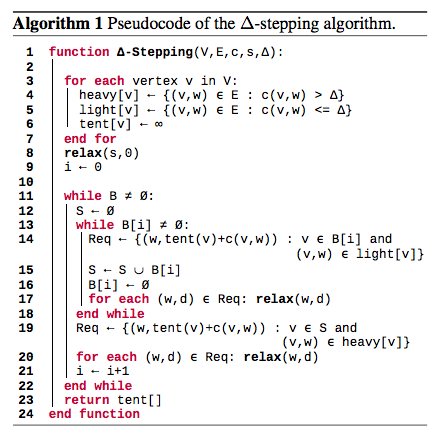
\includegraphics{algo_1.png}

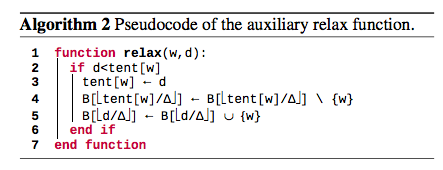
\includegraphics{algo_2.png}


\section{The implementation:}
\label{Algorithm:the-implementation}
Here is the code propposed for the first algorithm:

\begin{Verbatim}[commandchars=\\\{\}]
    function Deltastep(list,s,delta)
    C=Dict()
    V=Set()
    tent=Dict()
    B=Dict\PYGZob{}Any,Set\PYGZcb{}()
    E=Set()
    heavy=Dict()
    light=Dict()
    Req=[]
    pred=Dict()
    for item in list
        C[item[1],item[2]]=item[3]
        push!(V,item[1])
        push!(V,item[2])
        push!(E,[item[1],item[2]])
        heavy[item[1]]=[]
        heavy[item[2]]=[]
        light[item[1]]=[]
        light[item[2]]=[]
        tent[item[1]]=10000000000000
        tent[item[2]]=10000000000000
        pred[item[2]]=10000000000000
    end
    \PYGZsh{}println(\PYGZdq{}C=\PYGZdl{}C\PYGZdq{})
    for e in E
        v=e[1]
        w=e[2]
        if C[v,w]\PYGZgt{}delta
            push!(heavy[v],e)
        else
            push!(light[v],e)
        end
    end
    \PYGZsh{}println(\PYGZdq{}Heavy: \PYGZdl{}heavy\PYGZdq{})
    \PYGZsh{}println(\PYGZdq{}Light: \PYGZdl{}light\PYGZdq{})
    \PYGZsh{}println(\PYGZdq{}E=\PYGZdl{}E\PYGZdq{})
    relax(s,0,delta,B,tent,pred,1000000000)
    i=0
    while isempty(B)==false
        println(\PYGZdq{}B=\PYGZdl{}B\PYGZdq{})
        println(\PYGZdq{}tent=\PYGZdl{}tent\PYGZdq{})
        \PYGZsh{}Processing vertices from B[i]
        if haskey(B,i)==true
            S=Set()
            \PYGZsh{}Relax  recursively all light edges while they stay in B[i]
            while isempty(B[i])==false
                \PYGZsh{}Push to Req all light      edges from      vertices in B[i]
                Req=[]
                for v in B[i]
                    println(\PYGZdq{}v=\PYGZdl{}v\PYGZdq{})
                    for e in light[v]
                        println(\PYGZdq{}e  =\PYGZdl{}e\PYGZdq{})
                        push!(Req,[e[2],tent[v]+C[e[1]      ,e[2]],v])
                    end
                end
                \PYGZsh{}Update S
                union!(S,B[i])
                B[i]=Set()
                \PYGZsh{}Relax all  Req edges
                for r in Req
                    println(\PYGZdq{}r=\PYGZdl{}r\PYGZdq{})
                    relax(r[1],r[2],delta,B,ten     t,pred,r[       3])
                end
            end
            \PYGZsh{}Relax all heavy edges of vertices in S
            Req=[]
            delete!(B,i)
            for v in S
                for e in heavy[v]
                    push!(Req,[e[2],tent[v]+C[e[1],e[2]],v  ])
                end
            end
            for r in Req
                relax(r[1],r[2],delta,B,tent,pred,r[3])
            end
        end
        i=i+1
    end
println(\PYGZdq{}This is the answer: \PYGZdl{}tent\PYGZdq{})
return tent,pred
    end
\end{Verbatim}

The second algorithm was implemented in the following way:

\begin{Verbatim}[commandchars=\\\{\}]
function relax(w,d,delta,B,tent,pred,v)
    \PYGZsh{} println(\PYGZdq{}w : \PYGZdl{}w\PYGZdq{})
    if d\PYGZlt{}tent[w]
        old\PYGZus{}i=floor(tent[w]/delta)
        tent[w]=d
        if (haskey(B,old\PYGZus{}i)==true)
            delete!(B[old\PYGZus{}i],w)
        else
            \PYGZsh{} println(\PYGZdq{}Warning: In relax (w=\PYGZdl{}w,d=\PYGZdl{}d,delta=\PYGZdl{}delta), B[old\PYGZus{}i=\PYGZdl{}old\PYGZus{}i] not found\PYGZdq{})
        end
        \PYGZsh{}Add w to new bin and update its tent
        new\PYGZus{}i=floor(d/delta)
        if (haskey(B,new\PYGZus{}i)==false)
            B[new\PYGZus{}i]=Set()
            \PYGZsh{} println(\PYGZdq{}Warning: In relax (w=\PYGZdl{}w,d=\PYGZdl{}d,delta=\PYGZdl{}delta), allocated B[fld=\PYGZdl{}new\PYGZus{}i].\PYGZdq{})
        end
        push!(B[new\PYGZus{}i],w)
        tent[w]=d
        if (haskey(pred,w)==false)
            pred[w]=()
            pred[w]=v
            \PYGZsh{} println(\PYGZdq{}Warning: In relax (w=\PYGZdl{}w,d=\PYGZdl{}d,delta=\PYGZdl{}delta), allocated B[fld=\PYGZdl{}new\PYGZus{}i].\PYGZdq{})
        else
            pred[w]=v
        end
        \PYGZsh{} println(\PYGZdq{}The previous node visited was: \PYGZdl{}pred\PYGZdq{})
    end
end
\end{Verbatim}


\section{Path Function}
\label{Algorithm:path-function}
Some other functions were implemented. The following one, was implemented to retrieve the Path

\begin{Verbatim}[commandchars=\\\{\}]
function path(pred,w)
  v=w
  path = []
  while v\PYGZlt{}1000000000
        push!(path,v)
        \PYGZsh{}println(\PYGZdq{}\PYGZdl{}path\PYGZdq{})
        v = pred[v]
  end
  return reverse(path)
end
\end{Verbatim}


\section{Example:}
\label{Algorithm:example}
The following is an example of how to use the algorithm.

Let us start by setting up the graph. To do so let us define the following array:

\begin{Verbatim}[commandchars=\\\{\}]
graph=Array\PYGZob{}Int64\PYGZcb{}[]
push!(graph,[1,2,1])
push!(graph,[2,3,1])
push!(graph,[3,1,4])
push!(graph,[3,4,2])
push!(graph,[4,2,5])
\end{Verbatim}

\includegraphics{graph.gif}

Now we have a directed graph. Let us say we want to know the shortest path to each node from the vertice 2, we will do something like:

\begin{Verbatim}[commandchars=\\\{\}]
\PYG{n}{include}\PYG{p}{(}\PYG{l+s}{\PYGZdq{}}\PYG{l+s}{deltastep.jl}\PYG{l+s}{\PYGZdq{}}\PYG{p}{)}
\PYG{n}{include}\PYG{p}{(}\PYG{l+s}{\PYGZdq{}}\PYG{l+s}{relax.jl}\PYG{l+s}{\PYGZdq{}}\PYG{p}{)}
\PYG{p}{(}\PYG{n}{tent}\PYG{p}{,}\PYG{n}{pred}\PYG{p}{)}\PYG{o}{=}\PYG{n}{Deltastep}\PYG{p}{(}\PYG{n}{graph}\PYG{p}{,}\PYG{l+m+mi}{2}\PYG{p}{,}\PYG{l+m+mi}{1}\PYG{p}{)}
\end{Verbatim}

This is a simple code that runs over the graph, starting from the node 2 and with a delta of 1.

\includegraphics{deltastep.gif}

As is shown. It is obvious that going from node 2 to 2 has to have cost 0. The other nodes can be extracted very easy too.


\subsection{Parallel Delta-Stepping}
\label{Algorithm:parallel-delta-stepping}
The implementation provided for the Delta stepping algorithm is the following:

\begin{Verbatim}[commandchars=\\\{\}]
function Deltastep(list,s,delta)
    @everywhere rdc(d::Vector,i::Vector) = rdc(rdc(Dict(),d),i)
    @everywhere rdc(d::Dict,i::Vector) = begin d[i[1]] = []; d[i[2]] = [];d end
    @everywhere rdc(d::Dict,i::Dict) = merge!(d,i)
    @everywhere rdt(d::Vector,i::Vector) = rdt(rdt(Dict(),d),i)
    @everywhere rdt(d::Dict,i::Vector) = begin d[i[1]] = 1000000000000000;d[i[2]] = 1000000000000000; d end
    @everywhere rdt(d::Dict,i::Dict) = merge!(d,i)
    @everywhere rdcc(d::Vector,i::Vector) = rdcc(rdcc(Dict(),d),i)
    @everywhere rdcc(d::Dict,i::Vector) = begin d[i[1],i[2]] = i[3]; d end
    @everywhere rdcc(d::Dict,i::Dict) = merge!(d,i)
    @everywhere rds(d::Vector,i::Vector) = rds(rds(Set(),d),i)
    @everywhere rds(d::Set,i::Vector) = begin push!(d,i[1]);push!(d,i[2]); d end
    @everywhere rds(d::Set,i::Set) = union!(d,i)
    @everywhere rde(d::Vector,i::Vector) = rde(rde(Set(),d),i)
    @everywhere rde(d::Set,i::Vector) = begin push!(d,[i[1],i[2]]); d end
    @everywhere rde(d::Set,i::Set) = union!(d,i)
    heavy = @parallel (rdc) for item in list
      item;
    end
    light=@parallel (rdc) for item in list
        item;
    end
    tent= @parallel (rdt) for item in list
        item;
    end
    pred= @parallel (rdt) for item in list
        item;
    end
    C = @parallel (rdcc) for item in list
        item
    end
    V = @parallel (rds) for item in list
    item
    end
    E= @parallel (rde) for item in list
        item
    end
    B=Dict\PYGZob{}Any,Set\PYGZcb{}()
    Req=[]
    \PYGZsh{} println(\PYGZdq{}Heavy: \PYGZdl{}heavy \PYGZdq{})
    \PYGZsh{} println(\PYGZdq{}C=\PYGZdl{}C\PYGZdq{})
    for e in E
        v=e[1]
        w=e[2]
        if C[v,w]\PYGZgt{}delta
            push!(heavy[v],e)
        else
            push!(light[v],e)
        end
    end
    \PYGZsh{} println(\PYGZdq{}Light: \PYGZdl{}light  \PYGZdq{})
    \PYGZsh{} println(\PYGZdq{}E=\PYGZdl{}E\PYGZdq{})
    relax(s,0,delta,B,tent,pred,1000000000)
    i=0
    while isempty(B)==false
        \PYGZsh{} println(\PYGZdq{}B=\PYGZdl{}B\PYGZdq{})
        \PYGZsh{} println(\PYGZdq{}tent=\PYGZdl{}tent\PYGZdq{})
        \PYGZsh{} Processing vertices from B[i]
        if haskey(B,i)==true
            S=Set()
            \PYGZsh{} Relax recursively all light edges while they stay in B[i]
            while isempty(B[i])==false
                \PYGZsh{} Push to Req all light edges from vertices in B[i]
                Req=[]
                for v in B[i]
                    \PYGZsh{} println(\PYGZdq{}v=\PYGZdl{}v\PYGZdq{})
                    for e in light[v]
                        \PYGZsh{} println(\PYGZdq{}e=\PYGZdl{}e\PYGZdq{})
                        push!(Req,[e[2],tent[v]+C[e[1],e[2]],v])
                    end
                end
                \PYGZsh{} Update S
                union!(S,B[i])
                B[i]=Set()
                \PYGZsh{} Relax all Req edges
                for r in Req
                    \PYGZsh{} println(\PYGZdq{}r=\PYGZdl{}r\PYGZdq{})
                    relax(r[1],r[2],delta,B,tent,pred,r[3])
                end
            end
            \PYGZsh{} Relax all heavy edges of vertices in S
            Req=[]
            delete!(B,i)
            for v in S
                for e in heavy[v]
                    push!(Req,[e[2],tent[v]+C[e[1],e[2]],v])
                end
            end
            for r in Req
                relax(r[1],r[2],delta,B,tent,pred,r[3])
            end
        end

        i=i+1
    end
    println(\PYGZdq{}This is the answer: \PYGZdl{}tent\PYGZdq{})
    return tent,pred
end
\end{Verbatim}


\section{Some considerations}
\label{Algorithm:some-considerations}
One of the problems I found when trying to implement the algorithm in parallel, was the possibility to implement Shared memory data types for different structures like dictionaries, sets and others.

One of the solutions the community provided me when I asked on Stackoverflow was to create a set everywhere, populate it and in the end merge it. Doing this was helpful, however inefficient for memory allocations.

Let us see an example that clarifies this concept: We want to create a dictionary of sets. We want to set every vertex of the graph as a key and initialize it in parallel.

The first idea was simply to initialize a dictionary and then using \emph{@parallel}
populate it. Something like this:

\begin{Verbatim}[commandchars=\\\{\}]
julia\PYGZgt{} C=Dict()
julia\PYGZgt{} @parallel for item in a
                C[item[1],item[2]]=item[3]
           end
julia\PYGZgt{} println(\PYGZdq{}\PYGZdl{}C\PYGZdq{})
\end{Verbatim}

This was the result:

\includegraphics{dict.gif}

Again we face the problem of overwriting, from the race conditions. For this reason was necessary to implement the following way:

\begin{Verbatim}[commandchars=\\\{\}]
julia\PYGZgt{} @everywhere rdc(d::Dict,i::Vector)= begin d[i[1]] = length(a); d end
julia\PYGZgt{} @everywhere rdc(d::Vector,i::Vector) = rdc(rdc(Dict(),d),i)
julia\PYGZgt{} @everywhere rdc(d::Dict,i::Dict) = merge!(d,i)
julia\PYGZgt{} C = @parallel (rdc) for item in a
                item
            end
julia\PYGZgt{} println(\PYGZdq{}\PYGZdl{}C\PYGZdq{})
\end{Verbatim}

Implementing this way lead me to this desired result:

\includegraphics{paradict.gif}

Several solutions like this one were useful to parallel implementation.


\chapter{Images}
\label{Images:images}\label{Images::doc}\label{Images:id1}
The images in this project are very important. Specially because from them will be extracted the graphs that would allow us to run relevant  examples of  the algorihtm.

The Images package developed by Tim Holy, was extensively used. Let us provide some insights about how this work.

The first step is to load the image. The file should be on the same path you are executing Julia. You use the following command that would load the image as an array of pixels:

\begin{Verbatim}[commandchars=\\\{\}]
julia\PYGZgt{} using Images, Colors, FixedPointNumbers, ImageView
julia\PYGZgt{} img=load(\PYGZdq{}rose.png\PYGZdq{})
\end{Verbatim}

Now we can play with  and ``see'' the data:

\includegraphics{load.gif}

If you want to see the image you can use the following command:

\begin{Verbatim}[commandchars=\\\{\}]
\PYG{n}{julia}\PYG{o}{\PYGZgt{}}  \PYG{n}{view}\PYG{p}{(}\PYG{n}{img}\PYG{p}{)}
\end{Verbatim}

That would open an extra window showing


\includegraphics{rose.png}


\section{GrayScale}
\label{Images:grayscale}
Now we can convert this image to gray scale, so it is easy to handle for calculations.

{\color{red}\bfseries{}\textbar{}rosegray\textbar{}}


\section{Gradient}
\label{Images:gradient}
Now we can calculate gradient using the function from Images

\begin{Verbatim}[commandchars=\\\{\}]
julia\PYGZgt{} xx,yy=imgradients(A)
julia\PYGZgt{} c=(sqrt(xx.\PYGZca{}2+yy.\PYGZca{}2))
julia\PYGZgt{} view(c)
\end{Verbatim}


\includegraphics{gradient.png}

Now we need to find a way to reduce the cost of the middle of the images but make larger the cost of the border. To so I ran the following code:


\section{Cost}
\label{Images:cost}
\begin{Verbatim}[commandchars=\\\{\}]
julia\PYGZgt{} cost=1./(c.+1)
julia\PYGZgt{} view(cost)
\end{Verbatim}


\includegraphics{cost.png}

Now if you go and see the cost of the borders they will be smaller thant those outside (they will be around 1). Therefore we will have the way to form the shortest path as the border of the image.

\includegraphics{costvi.gif}

Now we are ready to set up the graph.


\chapter{Set Up the graph.}
\label{setup:setup}\label{setup:set-up-the-graph}\label{setup::doc}
In the last section I explained how to extract information from a picture and more important how to transform that information in order to make it relevant for our purposes.

In this section I will explain how I build the graph out of the image.

The directed graph we are trying to set is described by a list of items where each item has the following items (V1,V2, C) where V1 is connected with V2 (in that direction) and C is the cost of going from V1 to V2.


\section{Pixels, vertex and edges}
\label{setup:pixels-vertex-and-edges}
The nodes of our graph would be given by each pixel of the image. In future releases we will reduce significatively the number of pixels to describe a picture. Right now for the rose example we will be dealing with around 200.000 nodes. Heavy enough to make our algorithm to go for around a minute before getting the answer. In the future the idea is reduce those nodes to the half using zooming or different staff.

The edges are therefore a bigger problem. Each pixel has eight neigbours (I considered up,down, left, right and the corners), so there are 8 edges defined for each pixel. Setting the set of edges from our graph to around a million edges! This is just a huge ammount of information. In the following releases this will be  reduced significatively, because this causes a poor performance of the application.


\section{Cost function}
\label{setup:cost-function}
As explained before the reciprocus of the gradient would be used to calculate the cost. Actually the cost would be given by the gradient in the ending pixel itself.


\section{Setup function}
\label{setup:setup-function}
The following code is used to setup the graph. The input is an image and the output is a graph in the structure previously explained.


\section{Example}
\label{setup:example}
The following example ran over the rose picture would show the bast number of edges created by this approach. This would change in future releases.

\includegraphics{setup.gif}


\chapter{Profiling the Performance:}
\label{profiling:profiling-the-performance}\label{profiling:profiling}\label{profiling::doc}
Julia has \emph{@time}, \emph{@elapsed} and  \emph{@allocated} profiling tools. The firs one, time the application and shows the memory allocations  but shows the result as well. The second one would only output the time and the third one would only output the memory allocations.

This code was implemented to time and measure the memory allocation of the algorithm.


\section{Code for serial}
\label{profiling:code-for-serial}
\begin{Verbatim}[commandchars=\\\{\}]
using Images, Colors, FixedPointNumbers, ImageView
img=load(\PYGZdq{}rose.png\PYGZdq{})
include(\PYGZdq{}setup.jl\PYGZdq{})
include(\PYGZdq{}deltastep.jl\PYGZdq{})
include(\PYGZdq{}relax.jl\PYGZdq{})
include(\PYGZdq{}path.jl\PYGZdq{})
graph=setup(img)
f=open(\PYGZdq{}output.txt\PYGZdq{},\PYGZdq{}w\PYGZdq{})
for i in [10,50,100,500,1000]
Time=@elapsed Deltastep(graph,5000,i)
Alloc=@allocated Deltastep(graph,5000,i)
write(f,\PYGZdq{}  Deltastep : \PYGZdl{}i Time Elapsed \PYGZdl{}Time Memory Allocations : \PYGZdl{}Alloc \PYGZbs{}n\PYGZdq{})
end
close(f)
\end{Verbatim}


\section{Code for parallel}
\label{profiling:code-for-parallel}
\begin{Verbatim}[commandchars=\\\{\}]
using Images, Colors, FixedPointNumbers, ImageView
addprocs()
img=load(\PYGZdq{}Imagenes/rose.png\PYGZdq{})
include(\PYGZdq{}setup.jl\PYGZdq{})
include(\PYGZdq{}relax.jl\PYGZdq{})
include(\PYGZdq{}path.jl\PYGZdq{})
include(\PYGZdq{}deltastepar.jl\PYGZdq{})
graph=setup(img)
f=open(\PYGZdq{}outputpar.txt\PYGZdq{},\PYGZdq{}w\PYGZdq{})
for i in [10,50,100,500,1000]
Time=@elapsed Deltastep(graph,5000,i)
Alloc=@allocated Deltastep(graph,5000,i)
write(f,\PYGZdq{}Image :\PYGZdl{}size  Deltastep : \PYGZdl{}i Time Elapsed \PYGZdl{}Time Memory Allocations : \PYGZdl{}Alloc \PYGZbs{}n \PYGZdq{})
end
close(f)
\end{Verbatim}


\chapter{Results}
\label{profiling:results}
Running the profiling tools on the super computer Stampede I obtained the following results:

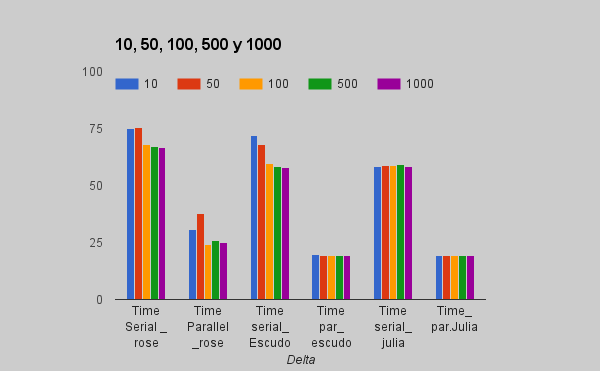
\includegraphics{experiment.png}

The parallel performance increased significatively. Even getting to a speed up of 2.9 which was closer to a linear performance.

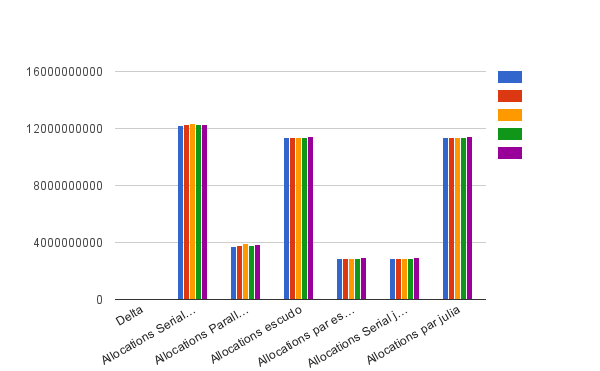
\includegraphics{allocations.png}

The results of the memory were kind of high in parallel. This is due to the used of the memory when I am creating the arrays in every node, and then merging the branches into the principal one.

Since julia is still on development (but now is reaching 0.5 dev version) is not available yet on Stampede. I use the binaries available to run it on stampede. But I could not run it with more than 3 process. Everytime I try to run it with more cores I got ``Could not allocate pools''.


\chapter{Analysis}
\label{profiling:analysis}
The performance observed on three processors of Stampede was about three times higher than in the serial code. This let us make conclusions on the weak scalling property of the code. However, due to the large size of the images, is important to notice that the performance was impacted great. In future releases this problem would be addressed. Specially using image compressing tools. that would let me describe the image very accurate with less pixels.

On the other hand, the problems I experienced running the code on Stampede shows that Julia is still on development and there are some compability problems in large scale computers. As well is necessary to increase the documentation coverage, specially for large scientific applications that requires more introduction for beginners.

However from the implementation is clear that Julia is a very dynamic language for programming. I have worked before in python, and it is easy to understand the new semantics given the proximity to that technical language in particular. In Images for instance, there is a comfortable and good proximity to matlab syntax.


\chapter{Demo}
\label{profiling:demo}
As a demo I ran the code, using the node img{[}11637{]} as the beginning node and the node img{[}154455{]}. Then following the guide provided in the \emph{quick reference} section I obtained the following image. I choose the view function of the gradient cost function so it is more visible the path found:

{\color{red}\bfseries{}\textbar{}rose1\textbar{}}


\chapter{Quick Reference}
\label{quickreference:quickreference}\label{quickreference::doc}\label{quickreference:quick-reference}
To launch the program right now you must follow the next steps.
\begin{enumerate}
\item {} 
Start julia.

\end{enumerate}

\begin{Verbatim}[commandchars=\\\{\}]
\PYGZdl{} Julia \PYGZhy{}p n
\end{Verbatim}
\begin{enumerate}
\setcounter{enumi}{1}
\item {} 
Load the packages needed:

\end{enumerate}

\begin{Verbatim}[commandchars=\\\{\}]
julia\PYGZgt{} using Images, Colors, FixedPointNumbers, ImageView
\end{Verbatim}
\begin{enumerate}
\setcounter{enumi}{2}
\item {} 
Include the functions needed.

\end{enumerate}

\begin{Verbatim}[commandchars=\\\{\}]
\PYG{n}{julia}\PYG{o}{\PYGZgt{}} \PYG{n}{Include}\PYG{p}{(}\PYG{l+s}{\PYGZdq{}}\PYG{l+s}{setup.jl}\PYG{l+s}{\PYGZdq{}}\PYG{p}{)}
\PYG{n}{julia}\PYG{o}{\PYGZgt{}} \PYG{n}{Include}\PYG{p}{(}\PYG{l+s}{\PYGZdq{}}\PYG{l+s}{deltastep.jl}\PYG{l+s}{\PYGZdq{}}\PYG{p}{)}
\PYG{n}{julia}\PYG{o}{\PYGZgt{}} \PYG{n}{Include}\PYG{p}{(}\PYG{l+s}{\PYGZdq{}}\PYG{l+s}{relax.jl}\PYG{l+s}{\PYGZdq{}}\PYG{p}{)}
\PYG{n}{julia}\PYG{o}{\PYGZgt{}} \PYG{n}{Include} \PYG{p}{(}\PYG{l+s}{\PYGZdq{}}\PYG{l+s}{path.jl}\PYG{l+s}{\PYGZdq{}}\PYG{p}{)}
\PYG{n}{julia}\PYG{o}{\PYGZgt{}} \PYG{n}{Include}\PYG{p}{(}\PYG{l+s}{\PYGZdq{}}\PYG{l+s}{color.jl}\PYG{l+s}{\PYGZdq{}}\PYG{p}{)}
\end{Verbatim}
\begin{enumerate}
\setcounter{enumi}{3}
\item {} 
Load the image and set it up.

\end{enumerate}

\begin{Verbatim}[commandchars=\\\{\}]
\PYG{n}{julia}\PYG{o}{\PYGZgt{}} \PYG{n}{img}\PYG{o}{=}\PYG{n}{load}\PYG{p}{(}\PYG{l+s}{\PYGZdq{}}\PYG{l+s}{Imagenes/rose.png}\PYG{l+s}{\PYGZdq{}}\PYG{p}{)}
\PYG{n}{julia}\PYG{o}{\PYGZgt{}} \PYG{n}{Graph}\PYG{o}{=}\PYG{n}{setup}\PYG{p}{(}\PYG{n}{img}\PYG{p}{)}
\PYG{n}{julia}\PYG{o}{\PYGZgt{}} \PYG{n}{tent}\PYG{p}{,}\PYG{n}{pred}\PYG{o}{=} \PYG{n}{deltastep}\PYG{p}{(}\PYG{n}{Graph}\PYG{p}{,}\PYG{n}{node}\PYG{p}{,}\PYG{n}{delta}\PYG{p}{)}
\PYG{n}{julia}\PYG{o}{\PYGZgt{}} \PYG{n}{path} \PYG{p}{(}\PYG{n}{pred}\PYG{p}{,} \PYG{n}{node}\PYG{p}{)}
\PYG{n}{julia}\PYG{o}{\PYGZgt{}} \PYG{n}{color}\PYG{p}{(}\PYG{n}{path}\PYG{p}{,}\PYG{n}{img}\PYG{p}{)}
\end{Verbatim}





\renewcommand{\indexname}{Index}
\printindex
\end{document}
